\graphicspath{{./figures}}

\section{Overview}

This project aims to design and implement a wireless communication system for a miniaturised satellite called a \textit{PocketQube} (PQ). The PocketQube standard was created to define physical and electronic requirements for so-called ``nano-satellites'', with the goal of easy integration of various sub-modules into one physical enclosure.

Nano-satellites can either be placed into orbit, or attached to a \textit{high-altitude balloon}. One common use-case of these balloons is to collect sensory information from the atmosphere, such as temperature and humidity readings. The goal of this project is to design a system that can be used in a balloon launch from the Saldanha Air Field, which may ultimately be done by the Stellenbosch Engineering department.

\begin{figure}[!htb]
  \begin{minipage}{.49\textwidth}
    \centering
    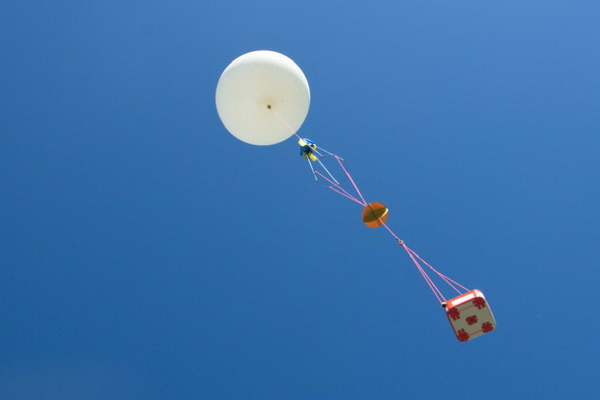
\includegraphics[width=0.95\linewidth]{balloonSat}
    \caption{A High-Altitude Balloon Carrying a Nano-Satellite Payload \cite{site-cyberBalloonLaunch}}
    \label{fig:balloonSat}
  \end{minipage}
  \begin{minipage}{.49\textwidth}
    \centering
    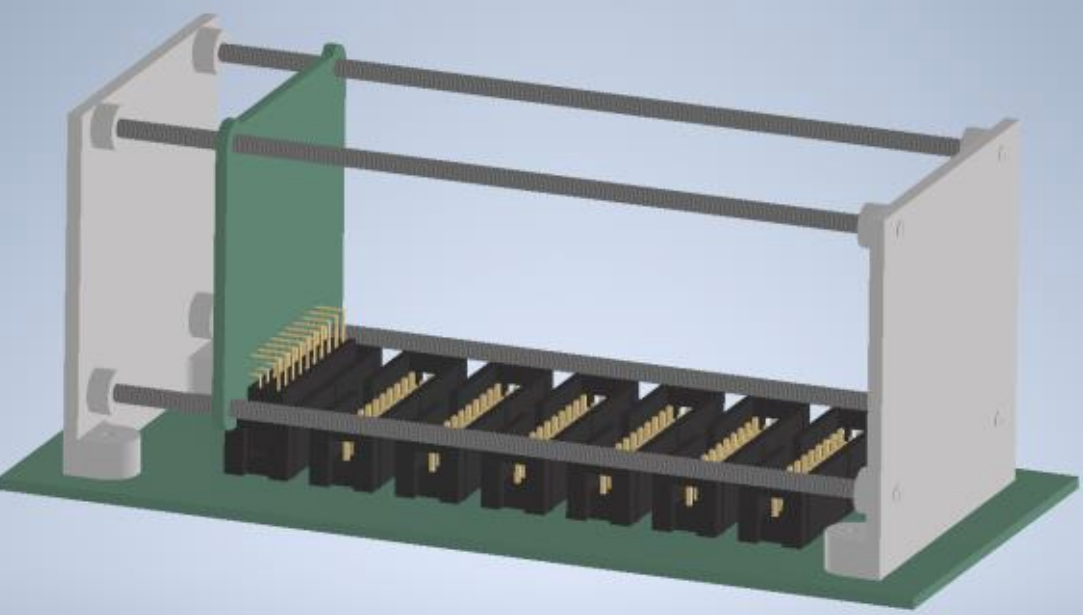
\includegraphics[width=0.99\linewidth]{pq_enclosure}
    \caption{A CAD Model of a Stellenbosch PocketQube Enclosure \cite{standard-pqsu}}
    \label{fig:pq_enclosure}
  \end{minipage}
\end{figure}

A satellite communication system includes both a ground station (GS), as well as a module on the satellite itself. The aim of this project is to establish a minimal prototype for both of these systems, so that future projects can refine the developed sub-systems. In this report, general system requirements are first listed, and a problem statement is drawn up. Then, a literature review is conducted to gather background information in the fields of interest. This includes an overview of the PocketQube standard, antenna theory, satellite tracking, and telecommunication theory. A systems level design is then done, which is followed by a more detailed design. Finally, the system is implemented and tested, the results are discussed, and potential improvements and work for future projects are listed.